\documentclass[twoside,10pt]{article}
\usepackage{amsmath,amsfonts,amsthm,fullpage,amssymb}
%\usepackage{mymath}
\usepackage{algorithm,amsmath,amssymb}
\usepackage{algorithmic}
\usepackage{graphicx, color}
\usepackage{url}


\begin{document}


\title{ISYE 6740 Homework 6\\ 
Spring 2021\\ 
\small Total 100 points + 10 bonus points.}
\date{}
\maketitle



%As usual, please submit a report with sufficient explanation of your answers to each the questions, together with your code, in a zip folder.

%----------------------------------------------------------------------------------

%feature selection (CV, bias-variance tradeoff), Boosting, random forest 

\begin{enumerate}

\item {\bf House price dataset.} (25 points)

The HOUSES dataset contains a collection of recent real estate listings in San Luis Obispo county and around it. The dataset is provided in RealEstate.csv. You may use ``one-hot-keying'' to expand the categorical variables.

The dataset contains the following useful fields (You may excluding the \textsf{Location} and \textsf{MLS} in your linear regression model). 

You can use any package for this question.

\begin{itemize}
\item Price: the most recent listing price of the house (in dollars).
\item Bedrooms: number of bedrooms.
\item Bathrooms: number of bathrooms.
\item Size: size of the house in square feet.
\item Price/SQ.ft: price of the house per square foot.
\item Status: Short Sale, Foreclosure and Regular.
\end{itemize}

\begin{enumerate}

\item (10 points) Fit the Ridge regression model to predict \textsf{Price} from all variable. You can use one-hot keying to expand the categorical variable \textsf{Status}. Use 5-fold cross validation to select the regularizer optimal parameter, and show the CV curve. Report the fitted model (i.e., the parameters), and the sum-of-squares residuals.  You can use any package.
 
\item (10 points) Use lasso to select variables. Use 5-fold cross validation to select the regularizer optimal parameter, and show the CV curve.  Report the fitted model (i.e., the parameters selected and their coefficient). Show the Lasso solution path. You can use any package for this. 

\item (5 points) Use elastic net to select variables. Report the fitted model (i.e., the parameters selected and their coefficient). Use  5-fold  cross validation to select the regularizer optimal parameter. You can use any package for this.

\end{enumerate}

\clearpage


\item  {\bf AdaBoost.} (25 points)

Consider the following dataset, plotting in the following figure. The first two coordinates represent the value of two features, and the last coordinate is the binary label of the data.
\begin{equation*}
\begin{split}
&X_1 = (-1, 0, +1), X_2 = (-0.5, 0.5, +1), X_3 = (0, 1, -1), X_4 = (0.5, 1, -1), \\
&X_5 = (1, 0, +1), X_6 = (1, -1, +1), X_7 = (0, -1, -1), X_8 = (0, 0, -1).
\end{split}
\end{equation*}

In this problem, you will run through $T = 3$ iterations of AdaBoost with decision stumps (as explained in the lecture) as weak learners.

\begin{enumerate}
\item (15 points) For each iteration $t = 1, 2, 3$, compute $\epsilon_t$, $\alpha_t$, $Z_t$, $D_t$ by hand (i.e., show the calculation steps) and draw the decision stumps on the figure (you can draw this by hand). 

\item (10 points) What is the training error of this AdaBoost? Give a short explanation for why AdaBoost outperforms a single decision stump.

\end{enumerate}


%vspace{-.2in}
\begin{figure}[h!]
\begin{center}
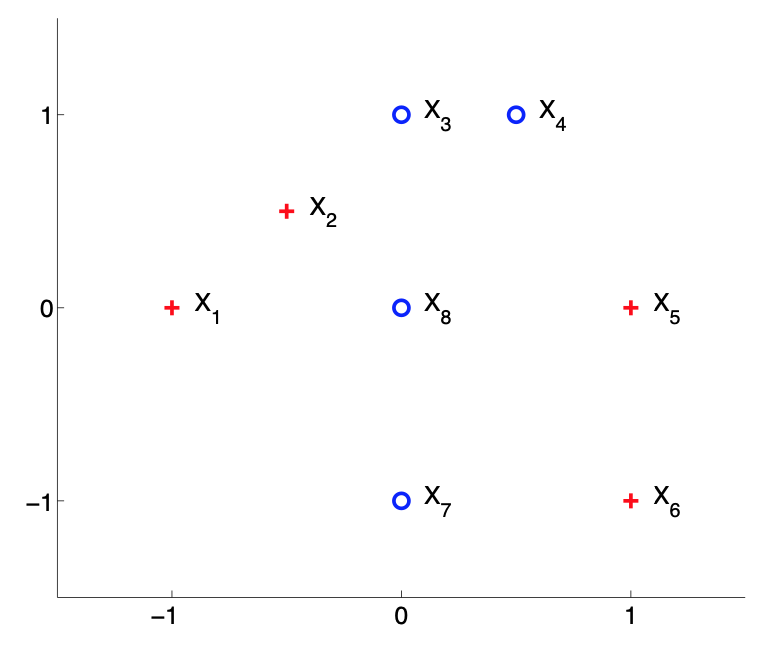
\includegraphics[width =.4 \textwidth]{hw}
\end{center}
%\caption{ A small dataset, for binary classification with AdaBoost.}
\end{figure}
\vspace{-.3in}

\begin{table}[h!]
\begin{center}
\caption{Values of AdaBoost parameters at each timestep.}
\vspace{0.1in}
\begin{tabular}{|c|c|c|c|c|c|c|c|c|c|c|c|}\hline
t & $\epsilon_t$ & $\alpha_t$ & $Z_t$ & $D_t(1)$ & $D_t(2)$ & $D_t(3)$ & $D_t(4)$ & $D_t(5)$ & $D_t(6)$ & $D_t(7)$ & $D_t(8)$ \\\hline
1 & & & & & & & & & & & \\
2 & & & & & & & & & & &\\
3 & & & & & & & & & & & \\\hline
\end{tabular}
\end{center}
\end{table}







\clearpage

\item {\bf Random forest and one-class SVM for email spam classifier} (25 points)

Your task for this question is to build a spam classifier using the UCR email spam dataset \url{https://archive.ics.uci.edu/ml/datasets/Spambase} came from the postmaster and individuals who had filed spam. Please download the data from that website. The collection of non-spam emails came from filed work and personal emails, and hence the word \textsf{'george'} and the area code \textsf{'650'} are indicators of non-spam. These are useful when constructing a personalized spam filter. You are free to choose any package for this homework. Note: there may be some missing values. You can just fill in zero.

\begin{enumerate}

\item (5 points) Build a CART model and visualize the fitted classification tree.

\item (10 points) Now also build a random forest model. Partition the data to use the first 80\% for training and the remaining 20\% for testing. Compare and report the test error for your classification tree and random forest models on testing data. Plot the curve of test error (total misclassification error rate) versus the number of trees for the random forest, and plot the test error for the CART model (which should be a constant with respect to the number of trees). 

\item (10 points) Now we will use a one-class SVM approach for spam filtering. Partition the data to use the first 80\% for training and the remaining 20\% for testing. Extract all {\it non-spam} emails from the training block (80\% of data you have selected) to build the one-class kernel SVM using RBF kernel (you can turn the kernel bandwidth to achieve good performance). Then apply it on the 20\% of data reserved for testing (thus this is a novelty detection situation), and report the total misclassification error rate on these testing data. 

\end{enumerate}



\clearpage 

\item {\bf Locally weighted linear regression and bias-variance tradeoff.} (25 points)

Consider a dataset with $n$ data points $(x_i, y_i)$, $x_i \in \mathbb R^p$, following the following linear model
\[
y_i = {\beta^*}^T x_i + \epsilon_i, \quad i = 1, \ldots, n,
\]
where $\epsilon_i \sim \mathcal N(0, \sigma_i^2)$ are independent (but not identically distributed) Gaussian noise with zero mean and variance $\sigma_i^2$.

 
\begin{enumerate}

\item (5 points) Show that the ridge regression which introduces a squared $\ell_2$ norm penalty on the parameter in the maximum likelihood estimate of $\beta$ can be written as follows
\[
\hat \beta (\lambda) = \arg \min_{\beta} 
\left\{
(X \beta - y)^T W (X \beta - y) + \lambda \|\beta\|_2^2
\right\}
\]
for property defined diagonal matrix $W$, matrix $X$ and vector $y$. 


\item (5 points) Find the close-form solution for $\widehat {\beta}(\lambda)$ and its distribution conditioning on $\{x_i\}$.

\item (5 points) Derive the bias as a function of $\lambda$ and some fixed test point $x$.

\item (5 points) Derive the variance term as a function of $\lambda$.

	⁃	\item (5 points) Now assuming the data are one-dimensional, the training dataset consists of two samples $x_1 = 1.5$ and $x_2 = 1$,  and the test sample $x = 0.5$. The true parameter $\beta_0^* = 1$, $\beta_1^* = 0.5$, the noise variance is given by $\sigma_1^2 = 2$, $\sigma_2^2 = 1$. Plot the MSE (Bias square plus variance) as a function of the regularization parameter $\lambda$. 

\end{enumerate} 


\clearpage
\item {\bf Medical imaging reconstruction.} (10 points)

In this problem, you will consider an example resembles medical imaging reconstruction in MRI.  We begin with a true image image of dimension 50 $\times$ 50 (i.e., there are 2500 pixels in total). Data is \textsf{cs.mat}; you can plot it first. This image is truly sparse, in the sense that 2084 of its pixels have a value of 0, while 416 pixels have a value of 1. You can think of this image as a toy version of an MRI image that we are interested in collecting.

Because of the nature of the machine that collects the MRI image, it takes a long time to measure each pixel value individually, but it's faster to measure a linear combination of pixel values. We measure $n$ = 1300 linear combinations, with the weights in the linear combination being random, in fact, independently distributed as $\mathcal{N}(0,1)$. Because the machine is not perfect, we don't get to observe this directly, but we observe a noisy version. These measurements are given by the entries of the vector
\[
y = A x + n,
\]
where $y \in \mathbb R^{1300}$, $A \in \mathbb R^{1300\times 2500}$, and $n \sim \mathcal N(0, 25\times I_{1300})$ where $I_n$ denotes the identity matrix of size $n\times n$. In this homework, you can generate the data $y$ using this model. 

Now the question is: can we model $y$ as a linear combination of the columns of $x$ to recover some coefficient vector that is close to the image? Roughly speaking, the answer is yes. 

Key points here: although the number of measurements $n$ = 1300 is smaller than the dimension $p$ = 2500, the true image is sparse. Thus we can recover the sparse image using few measurements exploiting its structure. This is the idea behind the field of \textit{compressed sensing}. 

The image recovery can be done using lasso
\[
\min_x \|y-Ax\|_2^2 + \lambda \|x\|_1.
\]
\begin{enumerate}
\item (5 points) Now use lasso to recover the image and select $\lambda$ using 10-fold cross-validation. Plot the cross-validation error curves, and show the recovered image. 
\item (5 points) To compare, also use ridge regression to recover the image:
\[
\min_x \|y-Ax\|_2^2 + \lambda \|x\|_2^2.
\]
Select $\lambda$ using 10-fold cross-validation. Plot the cross-validation error curves, and show the recovered image. Which approaches give a better recovered image?
\end{enumerate}



\end{enumerate}





\end{document}
